\documentclass[tikz,border=4pt]{standalone}
\usepackage{ctex}
\usepackage{amsmath}
\usetikzlibrary{calc, angles, quotes, decorations.markings, arrows.meta}
\begin{document}
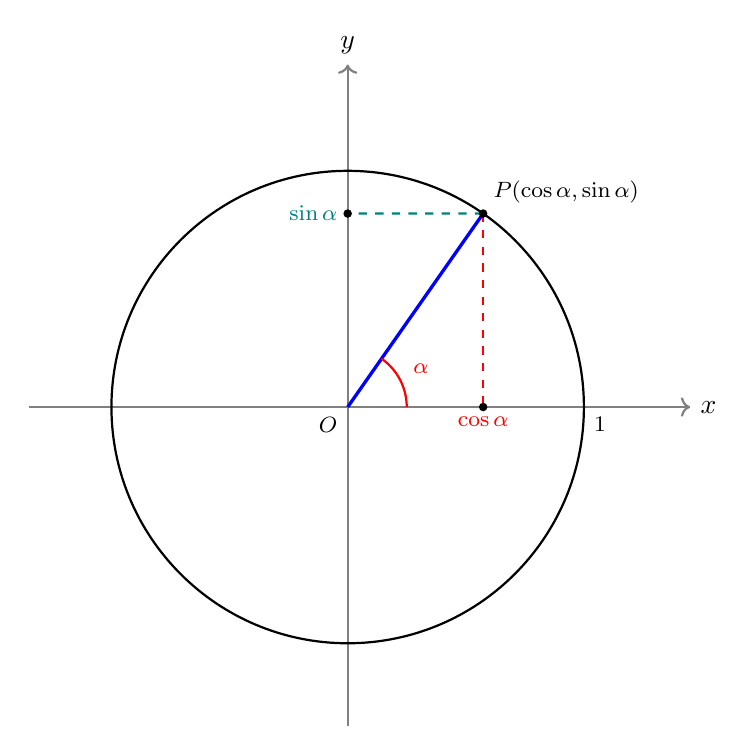
\begin{tikzpicture}[scale=3.0, thick]
  % 坐标轴
  \draw[->, gray] (-1.35,0) -- (1.45,0) node[right, black] {$x$};
  \draw[->, gray] (0,-1.35) -- (0,1.45) node[above, black] {$y$};
  % 单位圆
  \draw[black] (0,0) circle (1);
  % 角 alpha = 55°
  \def\ang{55}
  \coordinate (O) at (0,0);
  \coordinate (P) at ({cos(\ang)}, {sin(\ang)});
  \coordinate (X) at ({cos(\ang)}, 0);
  % 终边
  \draw[blue, very thick] (O) -- (P);
  % 角弧
  \draw[red, thick] (0.25,0) arc (0:\ang:0.25);
  \node[red, font=\footnotesize] at ({0.35*cos(\ang/2)}, {0.35*sin(\ang/2)}) {$\alpha$};
  % 投影
  \draw[red, dashed, thick] (P) -- (X);
  \draw[teal, dashed, thick] (P) -- (0,{sin(\ang)});
  % P 点
  \fill (P) circle (0.018);
  \node[above right, font=\footnotesize] at (P) {$P(\cos\alpha,\sin\alpha)$};
  % x 投影标
  \fill (X) circle (0.018);
  \node[below, font=\footnotesize, red] at (X) {$\cos\alpha$};
  % y 投影标
  \fill (0,{sin(\ang)}) circle (0.018);
  \node[left, font=\footnotesize, teal] at (0,{sin(\ang)}) {$\sin\alpha$};
  % 原点
  \node[below left, font=\footnotesize] at (O) {$O$};
  % 单位标
  \node[below right, font=\footnotesize] at (1,0) {$1$};
\end{tikzpicture}
\end{document}
